\chapterimage{portada2.jpg}
\chapter*{Repaso Estructura de Datos}
\vspace{140px}
\begin{flushright}
    \textit{Hash Table es una de las estructuras de datos fundamentales que todo Ingeniero de Software debe comprender muy bien, pues típicamente aplican en los proyectos que desarrollaremos. 
}
\end{flushright}

%software atributos de calidad relevantes por las que debiera tomar una decisión de diseño --> usar esta estructura de datos.

Los conjuntos son fundamentales en la ciencia de la computación para soportar a los algoritmos, los cuales deben realizar diferentes operaciones sobre estos (inserción, borrado, saber si está presente, entre otros) y de manera dinámica, por tanto estos conjuntos deben ser dinámicos.

En una implementación de un conjunto dinámico, cada elemento es representado por un objeto cuyos campos pueden ser examinados y manipulados si tenemos un puntero a este. Algunas implementación asumen que los campos de estos elementos son a su vez un conjunto o par de clave valor. Las  operaciones que se realizan sobre estos conjuntos pueden ser consultas u operaciones de modificación, tales como:
\begin{itemize}
\item $search(S,k)$ consulta que dado un conjunto $S$ y un valor $k$ retorna un puntero $x$ al elemento en $S$ tal que $key[x]=k$ o $NIL$ si ese elemento no pertenece a $S$. \item $insert(S,X)$ una operación de modificación que aumenta el conjunto $S$ con el elemento apuntado por $X$.  
\end{itemize}

Una tabla hash es una estructura de datos que implementa el tipo de dato abstracto Diccionario mediante la asociación de llaves con valores. Es una estructura de datos eficientes para realizar búsqueda mediante las llaves sobre todo cuando se almacenan grandes cantidades de datos. 


En esta unidad entenderemos
\begin{itemize}
\item  ¿Cómo funciona una tabla hash?
%\item Trazaremos  decisiones de diseño detallado hacia la calidad del software 
\item Aprenderemos a implementarlas
\item Conoceremos  Bibliotecas que existen para no rehacer la rueda
%\item Construiremos Pruebas unitarias
\item Revisaremos otras aplicaciones de las funciones hash
\end{itemize}

Muchas aplicaciones requieren un conjunto dinámico para soportar las operaciones de $INSERT$, $SEARCH$ y $DELETE$. Por ejemplo: Un compilador para mantener una tabla de símbolos, en que las claves de los elementos son string de caracteres arbitrarios que corresponden a los identificadores en el lenguaje.
%
Una hash table es una estructura de datos efectiva para implementar diccionarios. Aunque buscar un elemento en una hash table puede tomar $O(n)$ en su peor caso, en la práctica, bajo razonamiento razonable, el tiempo esperado podría ser O(1). 

Una hash table puede representarse como una generalización de un arreglo ordinario de pares clave valor.  Por ejemplo podríamos representarlo así
\begin{lstlisting}
hashtable = [("test1",1),("test2", 2),]
\end{lstlisting}
y obtener el valor asociado a la clave "test1"  mediante $data['test1']$ si y solo sí antes recorrí este arreglo y es comparada la clave buscada con el primer elemento del par clave-valor.  

Cuando el número total de claves almacenadas es pequeño, abordarlos con arreglos puede ser una alternativa efectiva pues la hash table usaría un arreglo de tamaño proporcional al número de claves actualmente almacenadas. En vez de usar las claves como índices del arreglo, los índices son calculados a partir de la clave. Esto genera riesgos, como por ejemplo de colisión de índices en que más de una clave mapea al mismo índice del arreglo.

\section{Preliminares}

Una hash table es una estructura de datos para almacenar un conjunto de ítemes del tipo $x=<clave, valor>$, de manera que podamos determinar rápidamente si un ítem está en el conjunto o no. 



Un ejemplo de uso de estas tablas son utilizados por los routers de Internet, los cuales sobreviven millones de ataques diarios. Ataques dirigidos querrán apoderarse de un slot de enrutamiento en particular según el interés, por lo que la clave para este ataque es descubrir la función de hash de manera de descubrir ese slot, y eventualmente modificarlo para dirigir el tráfico a un sitio malicioso. De ahí la \textbf{importancia de las funciones de hash - de que realmente sean aleatorias.}

La primera idea tras las tablas hash es implementarlas como arreglos: mapear la entrada a un entero que sea el índice de un arreglo. 
La idea básica es escoger una función de hash que mapee todo valor posible para el ítem $x$ - en particular para su clave $k$, a un entero pequeño $h(x)$. Sea $S$ el conjunto de ítemes. Si utilizamos la representación de arreglo $A$ de tamaño $m$, donde $m$ es mucho más pequeño que el tamaño de $S$, entonces una función de hash es cualquier función de la forma 
\begin{equation}
funcionhash: S \rightarrow \{0,1,\ldots, m-1\}
\end{equation}
la cual mapea todo valor posible en $S$ en un slot de la tabla hash $(A[funcionhash()]$. Si el tamaño de $S=m$ entonces deberíamos usar $funcionhash(x)=x$.


\begin{tcolorbox}[colback=gray!5!white,colframe=orange!60!gray,title=Ejercicio] 
Digamos que queremos almacenar cinco elementos cuyas claves respectivas son 28, 18, 10, 25, 41. ¿En qué casilla del siguiente arreglo irían sus potenciales valores si utilizamos una $funcionhash(k)=k  \% 13$ por ejemplo?
\begin{center}
\begin{tabular}{ |c | c | c |c | c | c|c | c | c|c | c | c|c| }
\hline 
0 & 1 & 2 & 3 & 4 & 5 & 6 & 7 & 8 & 9 & 10& 11&12 \\
\hline 
& & & & & & & & & & & & \\
\hline 
\end{tabular}
\end{center}
\end{tcolorbox}


\section{Colisiones}
El primer problema inmediato de este enfoque es que existen $2^31$ enteros posibles, necesitamos un gran arreglo para ubicar a cada potencial elemento, lo que siempre será menor que la cantidad de enteros que necesito que me genere la función hash para todos los potenciales elementos.
Claramente, tendremos un arreglo de menor tamaño, por ejemplo de tamaño $m$, que permita asignar elementos en el arreglo $A[funcionhash(k)\%m]$. 


\begin{tcolorbox}[colback=gray!5!white,colframe=orange!60!gray,title=Método de la división para seleccionar la función de hash] No es recomendable utilizar el \textit{método de la división}  $funcionhash(x)=x \% m$, pues cuando $m$ es una potencia de 2 no es una buena función. Libros recomiendan que $m$ sea primo, para evitar colisiones, pero incluso cuando es así, cualquier pad de ítemes cuya diferencia es un múltiplo entero de m colisionará; para todos los enteros $numero$ y $x$, $funcionhash(x)=funcionhash(x+am).$  
\end{tcolorbox}

%\todo{hacer un ejemplo}


De todos modos, dos ítemes $x$ e $y$ colisionan si sus valores hash son iguales: $funcionhash(x)=sfuncionhash(y)$. Teóricamente si sabemos la cantidad de elementos que tendrá esta estructura, es posible que se pueda encontrar una función de hash \textit{perfecta} que evite colisiones completamente. No importa la función de hash que escojamos. Es más, al menos $|S|/m$ ítemes colisionarán. E ahí la importancia de que la función nos asegure las menos colisiones además de tener maneras alternativas de resolverlas.




\subsection{Método 1: Encadenamiento}
Primera idea: implementarlo como una lista enlazada. 

En una tabla hash con encadenamiento, cada entrada en, $T[i]$ no contiene un ítem sino un puntero a una lista enlazada de todos los ítemes de la tabla cuyo valor de hash que les dio $T[i]$. Sea $largo(x)$ el largo de la lista $T[funcionhash(x)]$. Para ver si hay un ítem $x$ en la tabla, se escanea la lista completa. El tiempo requerido del peor caso para buscar $x$ es $O(1)$ para todo elemento en  $T[funcionhash(x)]$, u $O(1+largo(T))$ (esto mismo para insertar y borrar). 


Sea $U$ el universo de todas las claves. Pensemos que fuera el conjunto de todos los strings de tamaño 64 bits. En este caso $|U|=2^64$ claves, aunque sólo almacenaremos un subconjunto $S \in U$. Suponga que debemos almacenar a lo más $n$ elementos, que es mucho más pequeño que $|U|$, por tanto cada clave $k \in U$ está mapeado a uno de los n slots por una función hash. 
Supongamos que $n=5$ con una función de hash de $funcionhask(k)=(13k+2) \% 5$. Luego de la inserción de los elementos $\{1,2,4,7,8\}$ la tabla se ve así
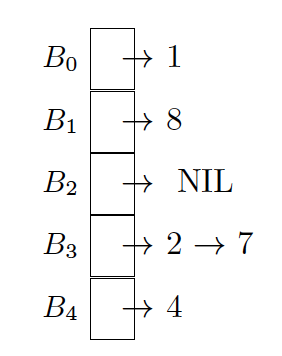
\includegraphics{Pictures/listaenlazada.png}


\begin{tcolorbox}[colback=gray!5!white,colframe=orange!60!gray,title=Ejercicio] Si escribimos una función hash para strings de largo exactamente igual a 2 en el rango [A,Z], entonces hay 26x26=676 combinaciones diferentes  de strings. Queremos implementar una función hash que produzca pocas colisiones, aunque pasado un tiempo vemos varias. Aplique la paradoja del cumpleaños y úsela para explicar el fenómeno. 
\end{tcolorbox}

Primero recordemos \textbf{el principio del casillero}: si hay más palomas que casilleros, entonces debe haber al menos un casillero con al menos dos palomas en él. Podemos decir que si n + 1 objetos se colocan en n cajas, entonces al menos una caja contiene dos o más objetos.

Dado que hemos escogido una tabla con tamaño casi 100, pero muchísimo más pequeño que 676, recordemos la \textbf{paradoja del cumpleaños}, que mapea la probabilidad de que dos personas tengan cumpleaños en un grupo de $n$ individuos seleccionados aleatoriamente. Para tener $100\%$ de probabilidad necesitamos 366 personas;  para una probabilidad de $99,9\%$ se necesitan 70 personas; para tener una probabilidad de $50\%$ se necesitan 23 personas. Si aplicamos esto a las colisiones en las tablas hash, entonces hay una alta probabilidad de que dos de nuestras 100 claves colisionen en este arreglo de tamaño 100. 




\begin{tcolorbox}[colback=gray!5!white,colframe=orange!60!gray,title=Eficiencia] De manera que las operaciones se implementen de manera eficiente, las claves deberían estar distribuidas uniformemente entre los slots de la hash table. Esperamos que todos los slots tengan a lo más un número constante de claves mapeadas a ellas, de maanera que las operaciones puedan ser realizadas en un tiempo constante. Para todo $h$, uno puede siempre producir un subconjunto de claves $S$ tal que todas ellas estén mapeadas a la misma ubicación. En ese caso, el tiempo será linear dependiente del número de claves y no constante como esperábamos.   
\end{tcolorbox}

%\color{red}

Sea $\alpha$ el factor de carga de la tabla hash $\alpha=\frac{n}{m}$.  Para garantizar el buen rendimiento de esta estructura de datos, este factor que se calcula como el número de elementos dividido por el tamaño del arreglo, debería ser menor que 1. Aunque se espera que sea menor que 0.75. Cuando un arreglo se va llenando, el factor de carga excede el valor predefinido, todos los valores almacenados en la tabla probablemente deban ser re-hasheados a una nueva tabla. 

\color{black}



\subsection{Direccionamiento abierto o hashing cerrado }


\begin{itemize}
    \item \textbf{sondeo lineal}
      \item \textbf{doble hasheo}
        \item \textbf{sondeo cuadrático}
\end{itemize}
\subsection{Importancia de la aleatoriedad de la función de hash para evitar colisiones}

Aleatoriedad ideal significa que una función de hash es escogida aleatoria pero \textit{uniformemente} de un conjunto de todas las funciones de $S a \{0,1,\ldots, m-1\}$. Por cada nuevo ítem, escogemos una función de hash para determinar el valor de hash. Lamentablemente, esto requeriría almacenar valores en una estructura separada que podría ser accedida usando  los ítemes en el conjunto. Por tanto, se buscan familias de funciones hash que sean suficientemente aleatorias para garantizar el buen rendimiento. Afortunadamente, la mayoría del análisis de hashing no requiere funciones hash aleatorias ideales. Por tanto las propiedades importantes que estas funciones deben cumplir son las siguientes:

\begin{itemize}
    \item \textbf{uniformidad}: una familia de funciones hash $H$ es uniforme si escogemos una función hash uniformemente de manera aleatoria de $H$ hace que todo valor hash sea probable para todo ítem en el universo: $P_{funcionhash \in H} [funcionhash(x)=i]=\frac{1}{m}$ para todo $x$ y para todo $i$.
    \item \textbf{universal}: una familia de funciones hash $H$ es universal, si para cualquier par de ítemes en el universo, la probabilidad de colisión es tan pequeña como sea posible: $P_{h \in H}[funcionhash(x)=funcionhash(y)] \leq \frac {1}{m}$ para todo $x \neq y$.
    
\end{itemize}
Ahora bien, usualmente basta con una versión más débil de universalidad y uniformidad.


\begin{itemize}
    \item \textbf{cerca universal}:  $P_{h \in H}[funcionhash(x)=funcionhash(y)] \leq \frac {2}{m}$ para todo $x \neq y$. Puede ser 2 u otra constante.
    
    \item \textbf{k uniformidad}: si razonamos respecto de grandes conjuntos de colisiones, decimos que para $k$ entero, una familia de funciones hash es 
 fuertemente $k$ universal o $k$ uniforme si para cualquier secuencia de $k$ claves disjuntas y cualquier secuencia de $k$ valores hash, la probabilidad de cada mapa de claves correspondiente al valor hash es $\frac {1}{m^K}$
\end{itemize}


Agloramiento ocurre cuando la función de hash provoca que claves comúnmente usadas tiendan a caer muy cerca unas de otras o de manera consecutiva, degradando el rendimiento de manera significativa, pues desperdiciamos otros espacios gastando recursos en resolver colisiones - sobre todo si usamos el sondeo lineal. 



\begin{tcolorbox}[colback=gray!5!white,colframe=orange!60!gray,title=Ejemplo de buena función hash] Suponiendo que queremos mantener una colección de unos 100 números de teléfonos. ¿Cuál sería una buena función de hash para este tipo de datos? \\
Una buena función sería por ejemplo los últimos dos dígitos o la suma de todos los dígitos. Una mala función serían los primeros dos dígitos probablemente pues probablemente tendremos muchos contactos del mismo lugar. De todos modos - siempre habrán colisiones. 
\end{tcolorbox}




\begin{tcolorbox}[colback=gray!5!white,colframe=orange!60!gray,title=Ejemplo en Strings] Dado que las palabras en español se construyen en base a las 27 letras (no consideraremos la ch o la ll), podemos asumir que la letra A tiene el número 0 y la letra Z tiene el número o índice 26. Por tanto nuestra función de hash puede descomponer las palabras en sus caracteres básicos y producir una buena salida de la función de hash a partir de la multiplicación de cada número asignado a cada caracter por 27 elevado al número de su posición (iniciando en 0). Por ejemplo, para la palabra "lala'', descomponiendo cada caracter lo llevamos a \{11,0,11,0\} y luego a $11*27^3+0*27^2+11*27^1+0*27^0$. 
\end{tcolorbox}











%vulnerabilidades
\section{Codificación y Pruebas unitarias}

\subsection{Nuestro primer código para una hash table}
\begin{lstlisting}
# Crear una tabla hash en python como una lista enlazada
HashTable = [[] for _ in range(10)]
  
# Función hash para retornar la vlave para todo valor 
def Hashing(keyvalue):
    return keyvalue % len(HashTable)
  
  
# Función para insertar valores a la hashtable 
def insert(Hashtable, keyvalue, value):
      
    hash_key = Hashing(keyvalue)
    Hashtable[hash_key].append(value)
    #print(value,keyvalue,hash_key)
    
    

# Función para mostrar la hashtable 
def display_hash(hashTable):
      
    for i in range(len(hashTable)):
        print(i, end = " ")
          
        for j in hashTable[i]:
            print("-->", end = " ")
            print(j, end = " ")
              
        print()
  

# quasimain
insert(HashTable, 20342454, 'Alumno1')
insert(HashTable, 21532231, 'Alumno2')
insert(HashTable, 20122321, 'Alumno3')
insert(HashTable, 19433423, 'Alumno4')
insert(HashTable, 21990334, 'Alumno5')
insert(HashTable, 20342432, 'Alumno6')
  
display_hash (HashTable)
\end{lstlisting}

Donde la salida de \code{display\_hash()} se ve así

\begin{lstlisting}
0 
1 --> Alumno2 --> Alumno3 
2 --> Alumno6 
3 --> Alumno4 
4 --> Alumno1 --> Alumno5 
5 
6 
7 
8 
9 
\end{lstlisting}














\subsection{Segunda versión -  Versión básica OO }
Ahora, usualmente es buena idea en el slot almacenar también la clave, de manera de poder realizar busquedas por clave. En esta sección además agregamos una función de hash menos trivial y que soporta Strings. 

\begin{lstlisting}
#!/usr/bin/env python3
# -*- coding: utf-8 -*-
"""
Created on Wed Nov 30 07:55:03 2022

@author: 
"""

############ una función hash para strings
def hash_function(key_str, size):

    fnhash=sum([ord(c) for c in key_str]) 
    print("valor función hash para la clave :" + key_str + ": " + str(fnhash))
    return fnhash% size


############ HashTable class
class HashTable:
    """ Esta hashtable usara string para claves 
    Ejemplo:
        ht = HashTable(10)
        ht.insertar('a', 1).insertar('b', 2).insertar('c', 3)
        ht['c'] = 30
    """

    def __init__(self, capacidad=1000):
        """ capacidad defaults to 1000. """

        self.capacidad = capacidad
        self.size = 0
        self._keys = []
        # Formato a almacenar: [ [ [key1, value], [key2, value] ], [ [key3, value] ] ]
       
        self.data = [[] for _ in range(capacidad)]

    def _buscar_por_clave(self, key, find_result_func):
        index = hash_function(key, self.capacidad)
        hash_table_cell = self.data[index]
        found_item = None
        for item in hash_table_cell:
            if item[0] == key:
                found_item = item
                break

        return find_result_func(found_item, hash_table_cell)

    def insertar(self, key, obj):
        """ insertar objeto con la clave entregada en la tabla hash.
        si existe entonces actualizar.
        sino adicionar. """

        def find_result_func(found_item, hash_table_cell):
            if found_item:
                found_item[1] = obj
            else:
                hash_table_cell.append([key, obj])
                self.size += 1
                self._keys.append(key)

        self._buscar_por_clave(key, find_result_func)
        return self

    def recuperar(self, key):
        """ Traer objeto asociado a la clave - debe ser un string sino debe generar un error. """

        def find_result_func(found_item, _):
            if found_item:
                return found_item[1]
            else:
                raise KeyError(key)

        return self._buscar_por_clave(key, find_result_func)

    def remover(self, key):
        """ removerr el objeto asociado con la clave. si lo encuentra el objeto sera retornado. sino se gatilla un error.  """

        def find_result_func(found_item, hash_table_cell):
            if found_item:
                hash_table_cell.remover(found_item)
                self._keys.remover(key)
                self.size -= 1
                return found_item[1]
            else:
                raise KeyError(key)

        return self._buscar_por_clave(key, find_result_func)




if __name__ == "__main__":
    print("creating hashtable test")
    ht = HashTable(10)
    print("capacidad: "+ str(ht.capacidad))
    print("insertando un elemento en una hashtable ")
    ht.insertar('lala', 1)
    print("ocupación:"+ str(ht.size))
    print("insertando un segundlo elemento en una  hashtable ")
    ht.insertar('b', 2)
    print("ocupación:"+ str(ht.size))
    print(str(ht.recuperar('lala')))
    print("valor hash para una clave lala:"+ str(hash_function('lala', 4)))
    
\end{lstlisting}



\subsection{Otros lenguajes de programación}

\begin{lstlisting}
    package hashtable;

/**
 *representación básica de un elemento a almacenar en la hashtable
 */
public class ElementoTablaHash {

    private Object key;
    private Object data;

    public ElementoTablaHash(Object key, Object data) {
        this.key = key;
        this.data = data;
    }

    public Object getData() {
        return data;
    }

    public Object getKey() {
        return key;
    }

}

\end{lstlisting}
\begin{lstlisting}
    package hashtable;

import java.util.ArrayList;
import java.util.LinkedList;



/**
 * crearemos una tabla hash como un arreglo de listas enlazadas
 * 
 */
public class TablaHash {
	//la implementamos como un arreglo de listas enlazadas
	private ArrayList<LinkedList<ElementoTablaHash>> cadenas;
	//con una capacidad máxima que no cambia.
    public final static int CAPACIDAD = 11;
    //sabremos además cuantos elementos estamos apuntando desde cada slot del arreglo
    private ArrayList<Integer> largoCadena;

    private int index;

    private int size;
   
    public TablaHash() {

        cadenas = new ArrayList<LinkedList<ElementoTablaHash>>(CAPACIDAD);
        largoCadena = new ArrayList<Integer>(CAPACIDAD);

        for (int i = 0; i < CAPACIDAD; i++) {
            cadenas.add(new LinkedList<ElementoTablaHash>());
            largoCadena.add(0);
        }

        size = 0;
    }
    
    /**
     * 
     * @return promedio del factor de carga
     */
    public double promedioFactorCarga() {
        double sum = 0.0;
        for (int i = 0; i < CAPACIDAD; i++) {
            sum += largoCadena.get(i);
        }
        return sum/CAPACIDAD;
    }

    
    /**
     * retorna un valor hash para una clave dada.
     * Sólo enteros o string son actualmente soportados. 
     * @param key la clave a ser hasheada. Debe ser Integer o String.
     * @return el valor hash para la clave 
     */
    private static int hash(Object key) {
        Class keyClass = key.getClass();
        if ( keyClass == Integer.class )
            return integerHash((Integer)key);
        else if ( keyClass == String.class )
            return stringHash((String)key);
        else
            throw new IllegalArgumentException("Hashing no soportado para " + keyClass);
    }
    /**
     * 
     * @param key la clave Integer a ser hasheada
     * @return el valor hash para la clave 
     */
    private static int integerHash(Integer key) {
        
        return key%CAPACIDAD;
    }

    /**
     * tarea 0 retorna el valor hash para una clave key de tipo String. 
     * @param key el String a ser hasheado 
     * @return el valor hash para la key 
     */
    private static int stringHash(String key) {
        // you must provide
        return 0;
    }
    	
   
    /**
     * Insertar una elemento en la tabla hash. 
     * @param elemento a ser insertado
     */
    public void insert(ElementoTablaHash elemento) {
        //calculamos el valor hash - recordemos buenas prácticas
    	index = hash(elemento.getKey());
    	//nos ubicamos en el slot de la lista enlazada
        LinkedList<ElementoTablaHash> candena = cadenas.get(index);
        //lo adicionamos al inicio
        candena.addFirst(elemento);
        //al contador de largo de la lista que apunta ese slot le sumamos uno más
        largoCadena.set(index, largoCadena.get(index)+1);
        //y por supuesto aumentamos los elementos que tenemos contenidos en nuestra hashtable
        size++;
    }
    
    /**
     * Limpiar la hashtable
     */
    public void clear() {
        for (int i = 0; i < CAPACIDAD; i++) {
            cadenas.get(i).clear();
            largoCadena.set(i, 0);
        }
        size = 0;
    }

    /**
     * Encontrar un elemento en la tabla hash dada una clave. 
     * @param key la clave a ser buscada. Debe ser entero o string.
     * @return el elemento con esta clave si existe. Sino null.
     */
    public ElementoTablaHash search(Object key) {
        // Tarea1
    	
        return null;
    }

    /**
     * Intenta remover un elemento de esta tabla hash. Se retorna true si el elemento se remueve y falso sino. 

     * @param elemento el elemento a ser removido
     * @return verdadero si el elemento se remueve
     */
    public boolean remove(ElementoTablaHash elemento) {
        // tarea 2
        return false;
    }

 
   
    /**
     * Calcula la desviación estándar para el largo promedio de la tabla 
	 * Una buena función de hash minimiza la desviación
     * @return la desviación estándar 
     */
    public double standardDeviation() {
        double mean = promedioFactorCarga();
        double sum_of_squares = 0.0;
        for (int i = 0; i < CAPACIDAD; i++) {
            sum_of_squares += Math.pow(largoCadena.get(i) - mean, 2);
        }
        return Math.sqrt(sum_of_squares/CAPACIDAD);
    }

    /**
     * Retorna el arreglo de largos de cadenas 
     * @return el arreglo de largos de cadenas 
     */
    public ArrayList<Integer> getChainLengths() {
        return largoCadena;
    }

    /**
     * Retorna el tamaño de la tabla, es decir los elementos en esta 
     * @return el tamaño de la tabla,
     */
    public int getSize() {
        return size;
    }

    /**
     * Recupera el indice del último slot de la tabla hasheado
     * @return el índice del último slot hasheado 
     */
    public int getIndex() {
        return index;
    }
    
    

}

\end{lstlisting}

\begin{lstlisting}
    package hashtable;

public class HashTableTest {

	public static void main(String[] args) {
		TablaHash th = new TablaHash();
		ElementoTablaHash eth = new ElementoTablaHash(5, "lala");
		
		th.insert(eth);
		eth = new ElementoTablaHash(10, "lola");
		th.insert(eth);
		eth = new ElementoTablaHash(20, "lolo");
		th.insert(eth);
		System.out.println("test");

	}

}

\end{lstlisting}

\subsection{Usando Bibliotecas}
Java provee una interfaz \code{Map} y muchas implementaciones de esta. La \code{interface Map<K,V>} es un objeto que mapea claves de tipo \code{K} a valores de tipo \code{V}, donde tanto \code{K} como \code{V} son tipos genéricos. Un \code{Map} no puede tener claves duplicadas; cada clave puede mapear a lo más un valor. Métodos:
\begin{itemize}
    \item \code{put(K key, V value)} asocia el valor especificado con la clave especificada. Retorna el valor previo asociado con la clave o nulo si no lo hubiera. 
\item \code{get(Object key)} retorna el valor al cual la clave esta mapeada o nulo de no haber. 
\item \code{remove(Object key)} remueve el mapeo de una clave en el mapa. Retorna el valor previo asociado con la clave o nulo de no haber. 
\item \code{Set<K> keySet()} retorna un conjunto de las claves contenidas en el mapa. 
\end{itemize}

Ahora bien, \code{class Hashtable<K,V> implements Map<K,V>} implementa una tabla Hash, que mapea claves a valores. Una clave o valor puede ser todo objeto no nulo.
Para almacenar exitosamente en una tabla hash, los objetos usados como claves deben implementar el método \code{hashCode} e \code{equal}.


A diferencia de lo anterior, Java oculta los detalles de implementación de una hashtable. 
\begin{lstlisting}

package cl.estructuradatos;

import java.util.Enumeration;
import java.util.Hashtable;

public class HashTableStrings {
	public static void main(String[] args) {
		 
		Enumeration names;
		String key;
	 
	   //Crear una hashtable
	   Hashtable<String, String> hashtable = 
	              new Hashtable<String, String>();
	 
	   // poblar la hashtable
	   
	   hashtable.put("0929306406","Horowitz");
	   hashtable.put("0201514257","Sedgewick");
	   hashtable.put("0201000237","Aho");
	   hashtable.put("8177584235","Kruse");
	 
	   //mostrar los elementos
	   names = hashtable.keys();
	   while(names.hasMoreElements()) {
	      key = (String) names.nextElement();
	      System.out.println("isbn-10: " +key+ " & Autor: " +
	      hashtable.get(key));
	   }
	   
	   //buscar un elemento por clave
	   String claveBuscada = "0929306406";
	   names = hashtable.keys();
	   while(names.hasMoreElements()) {
	      key = (String) names.nextElement();
	      
	      if (key.compareTo(claveBuscada)==0) {
	    	  System.out.println("encontrado valor asociada a clave: " +key+ 
                                    ":"+ hashtable.get(key));
	    	  break;
	      }
	      
	   }
	   //borrar clave valor "0201000237","Aho")
	   hashtable.remove("0201000237");
	   //just checking 
	   //mostrar los elementos
	   names = hashtable.keys();
	   while(names.hasMoreElements()) {
	      key = (String) names.nextElement();
	      System.out.println("isbn-10: " +key+ " & Autor: " +
	      hashtable.get(key));
	   }
	   //actualizar valor
	   hashtable.put("0201514257","Sedgewick***");
	   System.out.println("======================");
	 //just checking 
	   //mostrar los elementos
	   names = hashtable.keys();
	   while(names.hasMoreElements()) {
	      key = (String) names.nextElement();
	      System.out.println("isbn-10: " +key+ " & Autor: " +
	      hashtable.get(key));
	   }
	 }
}
\end{lstlisting}

\begin{comment}
    
\subsection{Análisis de costo }
Asumir que el diccionario contiene $n$ entradas, la tabla tiene la capacidad $m$. Las colisiones son resueltas usando encadenamiento. ¿Cuál es el costo de \textbf{buscar} e \textbf{insertar}? Observar que el costo de \textbf{insertar} es al menos lo que cuesta \textbf{buscar}. Pues necesitamos chequear si una entrada con esa clave ya está en el diccionario. 

\end{comment}


%vulnerabilidades
\section{Aplicaciones}


Hay muchas razones por las que hashing es muy importante para las empresas, en particular para las que centran sus esfuerzos en la recuperación de información. En la práctica, el \textbf{tiempo de ejecución esperado es frecuentemente la medida más importante}, donde en teoría usualmente nos concentramos en el peor caso. 


Por ejemplo, supongamos que queremos asegurar que nuestros clientes al bajar un archivo particular desde nuestro sitio Web, este haya sido bajado correctamente
El Sitio Web provee un hash para el archivo y al bajarse se verifica que lo bajado es correcto por asegurarse de que el hash del archivo y el generado es el mismo.
Por tanto es muy importante que la función de hash sea sensible a pequeños cambios en el archivo
Ambos deben usar la misma función de hash.
Es por tanto la función de hash un medio para asegurar la integridad de los archivos, dado que con esta es posoble asegurar con algo mucho más simple de verificar, que el archivo no ha sido cambiado. 
Si analizamos esto, nos damos cuenta que en el día a día también usamos este concepto. Determinar si dos individuos son el mismo, basta con calcular una función de hash sobre esta (huellas dactilares) y verificar que son idénticas, lo que nos permite en este caso asegurar que son el mismo individuo. 
\begin{figure}[h!]
    \centering
    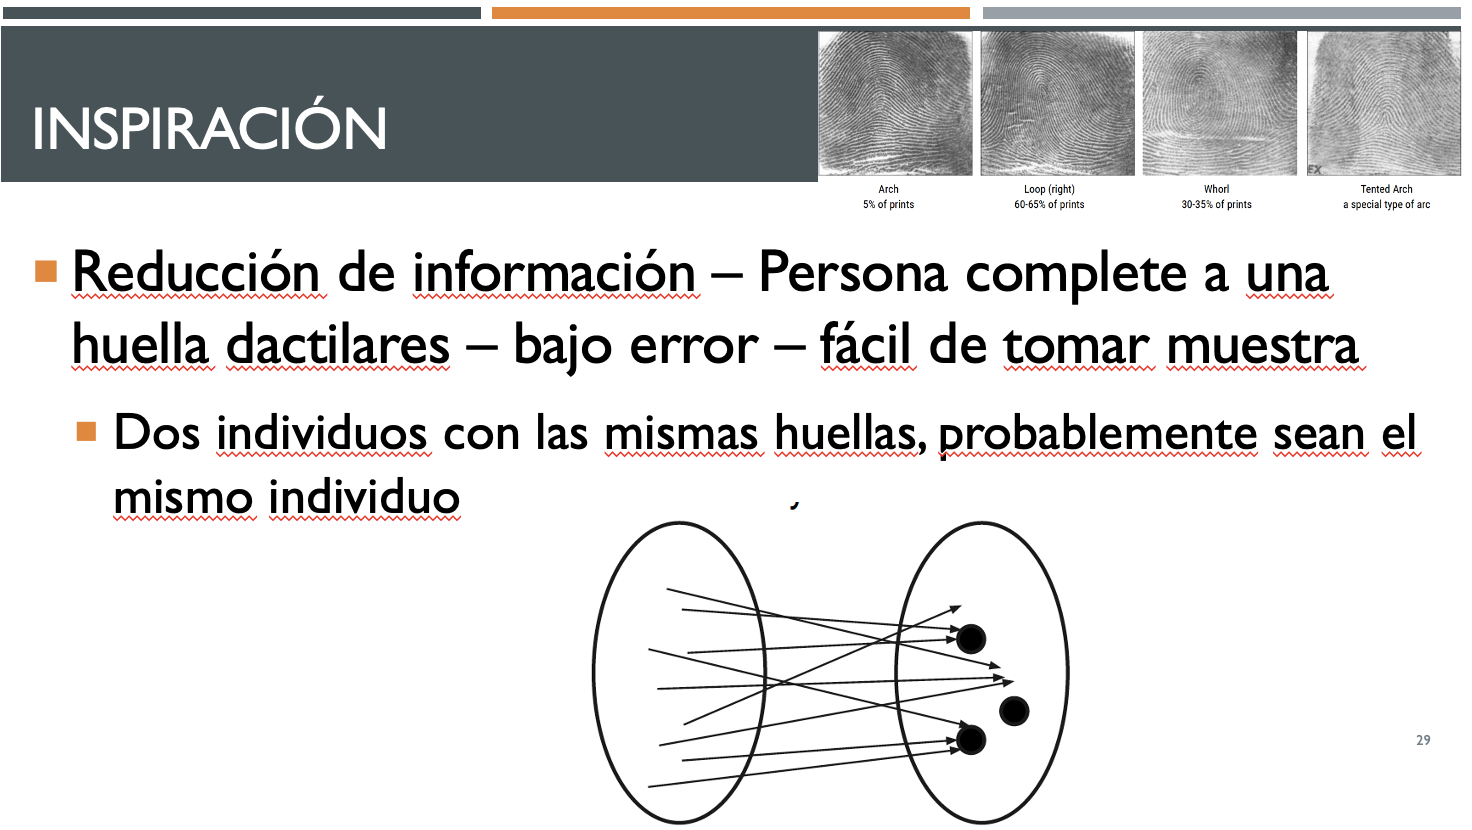
\includegraphics[width=0.5\textwidth]{Pictures/huellas.png}
    \caption{Caso trivial}
    \label{fig:my_label}
\end{figure}
Otro caso similar es si queremos detectar si un archivo es modificado, sin mantener una segunda copia de este. Se almacena un hash del archivo. Si queremos detectar modificaciones al archivo chequeamos el valor hash. Si una acción maliciosa quisiera reemplazar el archivo, sería muy difícil generar un segundo archivo con el mismo valor hash. Pues con ingeniería reversa uno puede intentar encontrar una manera. 
Supongamos además que estamos en un hospital donde encontramos en imagenología un examen complejo, y queremos saber si existen otros similares que ya hayan sido informados. Para ello, calculamos un valor hash por cada archivo. Si las imagenes similares mapean valores hash similares, entonces podemos ordenar los valores hash y chequear esos valores. 

Mucho hemos escuchado de fuerza bruta. Supongamos que queremos encontrar un substring de largo $k$ en un gran string de tamaño $n$. ¿Cuanto tiempo tomaría esto usando fuerza bruta? Una idea sería calcular un valor hash por cada substring de tamaño $k$. Para esta aplicación necesitamos las siguientes propiedades: los valores hash de $s_1 s_2 \ldots s_k$. 
Ver caso de desincriptacion de  claves \url{https://medium.com/spidernitt/introduction-to-timing-attacks-4e1e8c84b32b}

Estándar Wired equivalent privacy (WEP). WEP está construido sobre el algoritmo de encriptación RC4, creado para RSA en los 80. Con software libre en internet es fácil romper la encriptación de una red WEP en segundos. Dicen que usar WEP a veces es peor que no usar encriptación pues genera un relajo en los usuarios quienes tienen una seguridad falsa. Pues es como el agoritmo de cifrado de cesar. 

\begin{tcolorbox}[colback=gray!5!white,colframe=orange!60!gray,title=Actividad] 
Usemos sandbox de repl.it https://replit.com/languages/c y encripte su nombre 
\end{tcolorbox}
\begin{lstlisting}
#include <ctype.h>
#include <stdio.h>
#include <string.h>

#define SIZE 100

void encrypt(char str[], const char code[]) {
  int i, index;
  char c;

  for (i = 0; str[i] != '\0'; i++) {
    if (isalpha(str[i])) {
      c = tolower(str[i]);
      index = (int)c - 'a';
      str[i] = code[index];
    }
  }
}

void decrypt(char str[], const char code[]) {
  int i, index;
  char c;

  for (i = 0; str[i] != '\0'; i++) {
    if (isalpha(str[i])) {
      c = tolower(str[i]);

      /* find matching character */
      for (index = 0; index < 26; index++) {
        if (code[index] == c) {
          str[i] = (char)'a' + index;
        }
      }
    }
  }
}

int main() {
  char choice;
  char str[SIZE];
  char code[26] = {'t', 'f', 'h', 'x', 'q', 'j', 'e', 'm', 'u',
                   'p', 'i', 'd', 'c', 'k', 'v', 'b', 'a', 'o',
                   'l', 'r', 'z', 'w', 'g', 'n', 's', 'y'};

  printf("Seleccione una opción:\n");
  printf("1. Encriptar\n");
  printf("2. Desencriptar\n");
  scanf(" %c", &choice);

  if (choice == '1') {
    printf("Ingrese el texto a encriptar: ");
    scanf(" %[^\n]s", str);
    encrypt(str, code);
    printf("Texto encriptado: %s\n", str);
  } else if (choice == '2') {
    printf("Ingrese el texto a desencriptar: ");
    scanf(" %[^\n]s", str);
    decrypt(str, code);
    printf("Texto desencriptado: %s\n", str);
  } else {
    printf("Opción no válida\n");
  }

  return 0;
}

\end{lstlisting}
\begin{tcolorbox}[colback=gray!5!white,colframe=orange!60!gray,title=Historia - década de 1970] 
John Draper, un entusiasta de la tecnología y la telefonía, también conocido como "Captain Crunch" (Capitán Crunch), se hizo famoso por descubrir que el silbato que venía en las cajas de cereal Cap'n Crunch de la compañía Quaker Oats podía generar una señal de tono de 2600 Hz cuando se soplaba a través de él. Este tono de 2600 Hz resultó ser importante en el contexto de la telefonía de la época, ya que permitía el acceso gratuito a las líneas telefónicas de larga distancia, lo que se conoció como "phreaking".
El descubrimiento de John Draper sobre el tono de 2600 Hz y su capacidad para eludir sistemas de seguridad telefónica fue un precursor de la cultura hacker y la seguridad informática. El tono se convirtió en una herramienta para manipular sistemas telefónicos, y algunos consideran que fue un punto de partida para la exploración de la seguridad y la encriptación en la tecnología de la información.
Aunque la relación entre el cereal Cap'n Crunch y la encriptación es más anecdótica que directa, el apodo de "Captain Crunch" de John Draper se convirtió en parte de la historia de la tecnología y la seguridad informática, y su habilidad para descubrir cómo funcionaba el tono de 2600 Hz fue un precursor de la conciencia sobre la seguridad de las comunicaciones y la importancia de proteger la información.
\end{tcolorbox}


Para administrar las llaves y la autenticación - sistemas Cisco desarrollo el protocolo  LEAP (lightweight extensible authentication protocol), que podría usar WEP o  protocolo TKIP (Temporal Key Integrity Protocol) para setear las conexiones seguras. Dado que se conoce lo débil de WEP, TKIP ha emergido como el sustituto. Cisco en conjunto con Microsoft y RSA han creado PEAP (protected extensible authentication protocol) que difiere de LEAP en que requiere un certificado en el servidor. 

Controles para las debilidades de WEP:
\begin{itemize}
    \item protocolo de encriptación  CCMP: counter mode cipher block chaining message authentication code protocol - implementa el estándar IEEE 802.11i y provee seguridad mejorada usando en parte AES. 
    \item estándar \textbf{WPA (wifi protected access) } disponoble el 2003, usa encriptación AES fuerte para proteger la data de las redes y no tiene las mismas vulnerabilidades que WEP. WPA refiere al estándar estándar IEEE 802.11i .
    \item WPA2 oficialmente llamado estándar IEEE 802.11i-2004 del 2004 al 2018
    \item WPA3 puede operar en modo empresarial usando AES-256 en modo GCM
    \item WAP3 personal - usa AES-128 en modo CCM. 
\end{itemize}
Obviamente los dispositivos deben ser compatibles. por tanto desde el 2020 wpa3 se hizo mandatorio para obtener certificación de la alianza WiFi. 

Los tres estándares requieren ingresar una llave secreta compartida en la configuración de la red de todos los computadores de la red. También es posible reemplazar esto por entregar un usuario y clave única el cual puede ser proveido por un servicio para autenticar usuarios de manera remota (RADIUS introducida en 1991) el cual provee métodos para administrar autorización, autenticación y cuentas. (reemplazado por DIAMETER).